\documentclass[12pt,twoside]{article}

\usepackage{amsmath}
\usepackage[utf8]{inputenc}
\usepackage{template}
\usepackage{lipsum}

\usepackage{apacite}
\bibliographystyle{apacite}

\usepackage{Sweave}
\begin{document}
\Sconcordance{concordance:report.tex:report.Rnw:%
1 10 1 1 0 68 1 1 18 19 1 1 8 15 1 1 17 19 1 1 29 14 0 1 2 1 1 1 22 10 %
1 1 25 10 1 1 9 14 1 1 4 20 0 1 2 13 1}


\begin{titlepage}
\newcommand{\HRule}{\rule{\linewidth}{0.5mm}} 

\center % Center everything on the page

%	TITLE SECTION

\mbox{ }
\vspace{75mm}

%\HRule \\[0.8cm]
{ \Huge \bfseries \color{black}{Analysis of whistler weather data}}\\[0.4cm] 
%\HRule \\[1.5cm]

{\Large
\textsl{Stat 300 Project, Fall 2015}}

\bigskip
{\Large
by Nathan Esau, Ethan Sim, Benjamin Chan}

\vfill

%\vspace{15mm}
%\begin{figure}[!ht]
%\begin{center}
%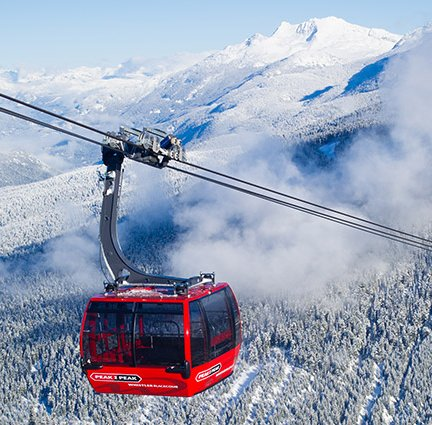
\includegraphics[width=0.9\textwidth]{tp_picture.jpg}
%\end{center}
%\end{figure}

%\vfill
%{\large
%Stat 300 Group Project \\ 
%\medskip
%Fall 2015}

\end{titlepage}

%\thispagestyle{firststyle}
%\noindent
%{\Large \textbf{Analysis of Whistler Weather Data}} 
%
%\medskip\noindent
{%\large \textsl{by Benjamin Chan, Ethan Sim and Nathan Esau}}

\section{Summary}

\subsection{Background}

In this study we analyze daily weather data from Whistler, BC. The variables analyzed were the amount of snow on the ground and the average temperature during each day.

\medskip\noindent
Our study was motivated by trying to answer the following questions:

\begin{enumerate}
\item When is the winter season? When does it start, peak and end?
\item How severe is the winter? How much snow is present at different points in the year? 
\item What trends exist in the data? What odd behaviors have shown up over the past nine years? 
\end{enumerate}

\subsection{Methods}

\noindent
To answer our questions, we used the following techniques:

\begin{enumerate}
\item Regression, to determine whether there was a trend in the snowfall data
\item Time series techniques, such as average smoothing, to compare different winter seasons
\item Correlation, to examine relationships between temperature and snowfall variables
\end{enumerate}

\subsection{Results}

We found that the amount of snow has been downward trending at a rate of -- 4.42 cm per year. The estimated start of winter in Whistler is December 3rd and the estimated end of winter is March 26th. The estimated length of winter is 114 days. A peak amount of snow of 86 cm usually occurs around February 12th. The average temperature during the winter is -0.98 degrees celsius. The shortest winter was the 2009--2010 season, which started on Nov 14th and ended on February 7th. This winter season also had the lowest peak amount of snow (58 cm). The average temperature and average snowfall during the winter had a correlation of -0.15.

\subsection{Interpretation}

We found that while temperature is very consistent year to year, the amount of snowfall has been showing a downward trend. We also showed that the 2009--2010 winter, in which Vancouver hosted the Olympics, had less snow and did not last as long as the other winter seasons. This was done by comparing the duration of snowfall, average snowfall and peak snowfall of the 2009--2010 winter to other winters. We defined winter as the period when snowfall is above is a given threshold.

By averaging different annual time series, we were able to determine the amount of snow present in Whistler at each point in the year. We found that snowfall can occur as early as September and as late as June in Whistler.

We also analyzed whether winters which are colder than average also tend to have above average snow. While the temperature and snowfall variables do exhibit some negative correlation, this does not mean that high snowfall is only caused by cold temperatures.

\section{Introduction}

Whistler Blackcomb is a Canadian resort town in the province of British Columbia, one of the largest ski resorts in North America. Whistler’s economy is highly dependent on the seasonality of snow as the main winter activities offered there are skiing and snowboarding. In July 2003, Whistler was selected to host the alpine skiing events for the 2010 Winter Olympics. However, 2010 was accompanied with an unusually mild winter. The lack of snow made it challenging to run some of the Winter Olympic activities. Given this kind of uncertainty, it would be helpful to have a rough estimate of when the Whistler winter season usually occurs and the peak time of snowfall.

Our weather data was obtained from \url{http://climate.weather.gc.ca/}. Data was recorded at an elevation of 657.80 metres, a longitude of 122$^{\circ}$57'17.400'' W and a latitude of 50$^{\circ}$ 07'44.001'' N over the period 2006 -- 2014. The data set contained the following variables

\begin{itemize}
\item Temperature -- minimum, maximum and mean temperature during each day
\item Snow on the ground 
\item Total precipitation 
\item Wind speed and direction
\end{itemize}

\vspace{-3mm}
\medskip The variables most relevant to answering our questions were the snow on the ground and the temperature. For temperature, we decided to use the mean temperature during each day, as we felt this is the most robust measure. We did not account for wind, due to the large number of missing and truncated values present, or for precipitation which we felt was not related to our question. 

We needed to perform some imputation for our variables. In particular, the snow on the ground during the summer months was not recorded, so we made the assumption that these was no snow on the ground at this point. Also, during the winter period when snow was not recorded we imputed the snow value from the previous day. Similarly, when the temperature was not recorded we imputed the temperature value from the previous day. During the winter, only a small portion of values ($<5\%$) were missing for these variables so this imputation should not have a large impact on our analysis.

Our overall goal was to understand the time series shown in Figure \ref{fig:basicts}. In this figure we have shown the two-week moving average for the amount of snow on the ground and the three-week moving average for the mean temperature.


\begin{figure}[!ht]
\begin{center}
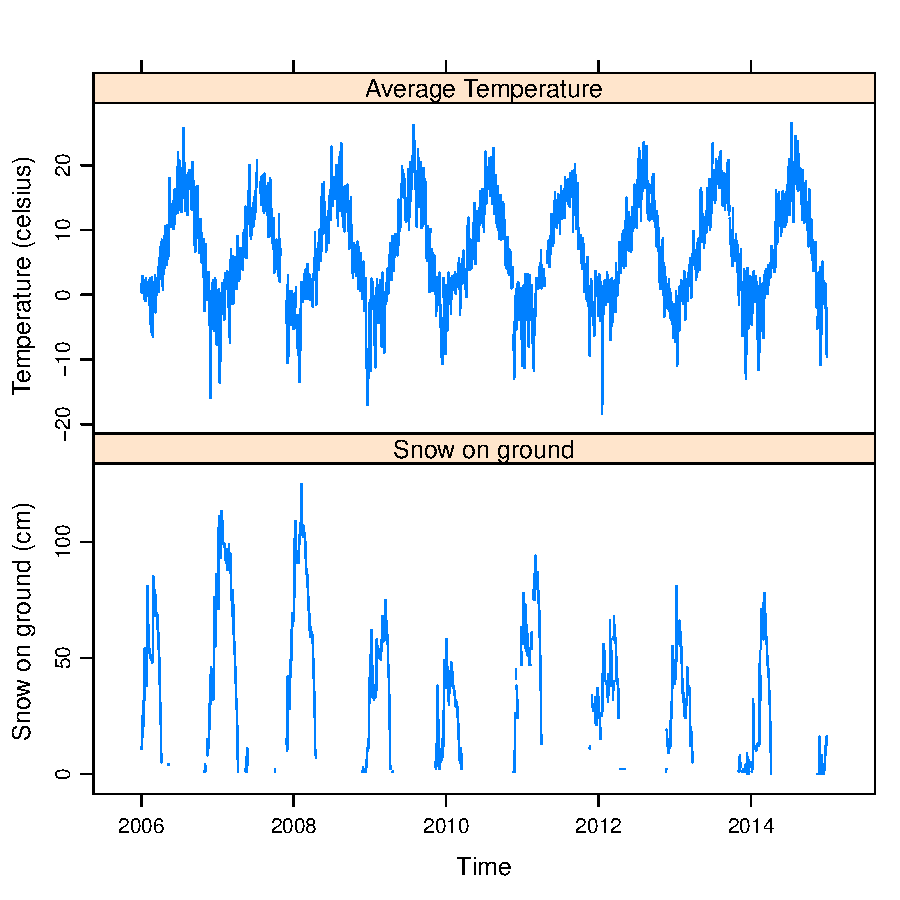
\includegraphics[width=0.8\textwidth]{report-basicts}
\end{center}
\vspace{-5mm}
\caption{Whistler weather data from 2006 -- 2014.}
\label{fig:basicts}
\end{figure}

\section{Methods and Results}

Our methods are divided into the following sections. First, we analyze whether a downward trend exists in the amount of snow during our observation period. Second, we average the annual time series and determine the minimum, maximum and average amount of snow present in Whistler at each day during the year. Finally, we compare the length and severity of each of the winter seasons. For the severity, we look at the average amount of snow and average temperature during the winter, and analyze whether these results are correlated in some way.

\subsection{Trend}

Linear regression was used to fit a trend for snowfall, as shown in Figure \ref{fig:snowtrend}. There is evidence that the amount of snow present in Whistler has been decreasing, as the slope coefficient is highly significant with $p$-value $< 0.001$. However, this downward trend is likely exaggerated due to the fact that we only have nine years of weather data. 

It is natural to wonder whether this downward trend is a result of rising temperatures (global warming). We found little evidence from our data to support this claim. For instance, the average temperatures (shown in Figure \ref{fig:basicts}) do not appear to be increasing  over time. When we tried fitting a trend line to these temperatures, the slope of the trendline indicated that temperatures have been increasing at a rate of $0.11$ degrees celsius per year. However, since the $p$-value $>$ for this slope was 0.01, we do not have too much evidence that temperatures have been increasing.


\begin{figure}[!ht]
\begin{center}
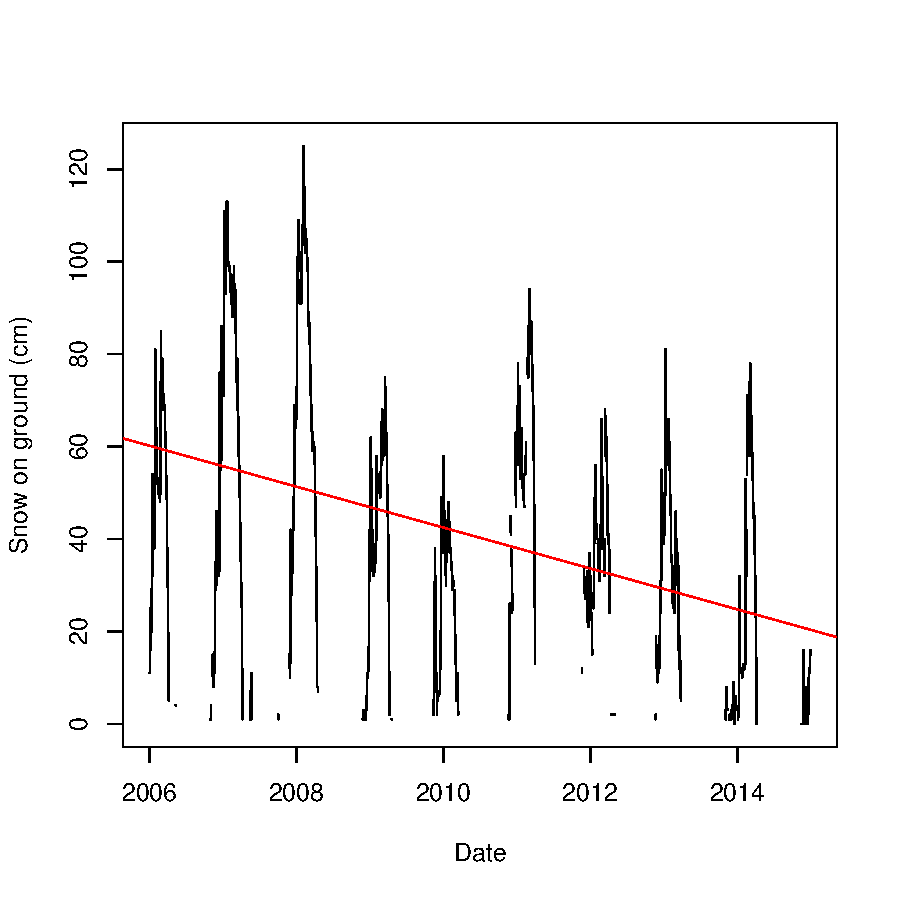
\includegraphics[width=0.7\textwidth]{report-snowtrend}
\end{center}
\vspace{-5mm}
\caption{Snowfall is trending downwards at a rate of 4.42 cm per year.}
\label{fig:snowtrend}
\end{figure}

\subsection{Average smoothing}

In order to determine how much snow is present at different points in the year, we averaged the nine years. One complication was that 2008 and 2012 were leap years. We needed each annual time series to be the same length in order to average them, so we removed February 29th of 2008 and 2012 from our data set.

The resulting minimum, maximum and average amount of snow at each day are shown in Figure \ref{fig:averagetsplot}. We have rearranged the dates to show the period July 1 -- June 30 rather than Jan 1 -- Dec 1. Notice that snowfall usually starts at the beginning of November and melts by the end of April. The amount of snow was recorded at an elevation of 657.8 metres, whereas the top of Whistler mountain has an elevation of 2,284 metres \cite{WhistlerBlackcomb}. This explains why the amount of snowfall in Figure \ref{fig:averagetsplot} is lower than one might expect for typical skiing conditions.

Figure \ref{fig:averagetsplot} also helps to convey some odd snowfall behavior. From the maximum line, we can see that it is possible to get snow at almost time during the year with the exception of July and August. From the minimum line, we can see that some years do not get any snow until December and have no snow mid-way into April.


\begin{figure}[!ht]
\begin{center}
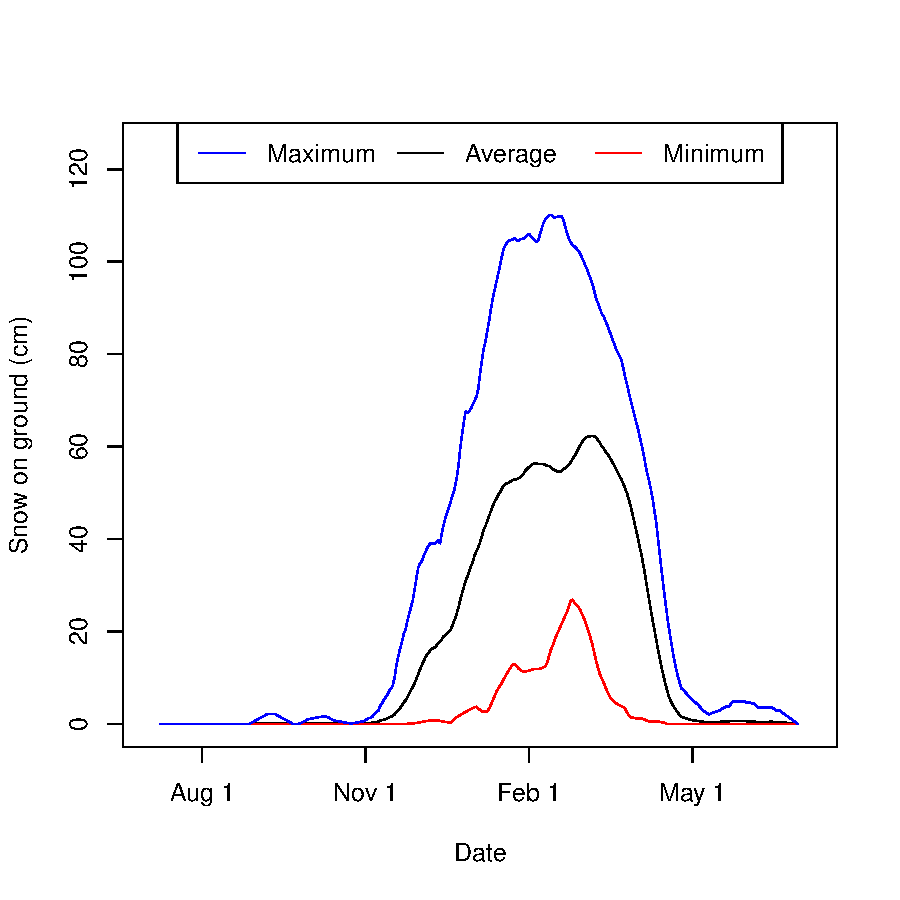
\includegraphics[width=0.7\textwidth]{report-averagetsplot}
\end{center}
\vspace{-8mm}
\caption{Amount of snow present at each day during the year based on period from 2006 -- 2014.}
\label{fig:averagetsplot}
\end{figure}

\subsection{Winter length and severity}

We also compared each of the winter seasons individually. Our assumption for the winter period was based on a snow threshold as shown in the equation below.
%
\begin{align*}
Winter &= \text{Period when } \text{7 day moving average of} \text{ snowfall} > \textsl{Threshold} \text{ (cm)}
\end{align*}

\medskip To check the robustness of our assumption, we tried varying the snowfall threshold over different values. The length of the winter under different thresholds is shown in Table \ref{tab:robustcheck}. Under each of these thresholds, the 2006--2007 and 2007--2008 are the longest winter seasons and 2009--2010 and 2013--2014 are the shortest. For the remainder of the analysis we decided to use a threshold of 15 cm.

% latex table generated in R 3.2.2 by xtable 1.8-0 package
% Sun Nov 29 22:29:55 2015
\begin{table}[ht]
\centering
\begin{tabular}{c|rrrrrrrr}
  \hline
Threshold (cm) & 06-07 & 07-08 & 08-09 & 09-10 & 10-11 & 11-12 & 12-13 & 13-14 \\ 
  \hline
10 & 145 & 138 & 108 & 93 & 136 & 143 & 121 & 87 \\ 
  15 & 137 & 135 & 103 & 85 & 128 & 136 & 99 & 87 \\ 
  20 & 134 & 132 & 101 & 78 & 125 & 126 & 94 & 55 \\ 
   \hline
\end{tabular}
\caption{Length of winter under a variety of thresholds} 
\label{tab:robustcheck}
\end{table}
\medskip
The dates associated with each of the winter  seasons are shown in Table \ref{tab:summarytable}. Notice that winter usually starts around December 3 and ends around March 26. However, the 2009--2010 was unusual, since it ended on February 7, much earlier than any of the other seasons. This means that by February 7, 2010, most of the snow was melted at the base of Whistler mountain. This explains why organizers had to bring in extra snow for the Olympics. The 2013--2014 winter was also unusual, only getting substantial snowfall by January 7.

% latex table generated in R 3.2.2 by xtable 1.8-0 package
% Sun Nov 29 22:29:55 2015
\begin{table}[ht]
\centering
{\small
\begin{tabular}{cccccccc}
  \hline
Winter & Start Date & End Date & Length & Peak Date & Peak Amt & Avg snow & Avg temp. \\ 
  \hline
2006-2007 & Nov 18 & Apr 4 & 137 days & Jan 19 & 113 cm & 72 cm & -0.56$^{\circ}$c \\ 
  2007-2008 & Nov 27 & Apr 11 & 135 days & Feb 7 & 125 cm & 73 cm & -1.23$^{\circ}$c \\ 
  2008-2009 & Dec 22 & Apr 4 & 103 days & Mar 17 & 75 cm & 48 cm & -1.8$^{\circ}$c \\ 
  2009-2010 & Nov 14 & Feb 7 & 85 days & Jan 2 & 58 cm & 30 cm & -1.17$^{\circ}$c \\ 
  2010-2011 & Nov 24 & Apr 1 & 128 days & Mar 5 & 94 cm & 59 cm & -1.31$^{\circ}$c \\ 
  2011-2012 & Nov 24 & Apr 9 & 136 days & Mar 15 & 68 cm & 38 cm & -0.37$^{\circ}$c \\ 
  2012-2013 & Dec 7 & Mar 16 & 99 days & Jan 9 & 81 cm & 41 cm & -1.26$^{\circ}$c \\ 
  2013-2014 & Jan 7 & Apr 4 & 87 days & Mar 6 & 78 cm & 37 cm & -0.17$^{\circ}$c \\ 
  Average & Dec 3 & Mar 26 & 114 days & Feb 12 & 86 cm & 50 cm & -0.98$^{\circ}$c \\ 
   \hline
\end{tabular}
}
\caption{Dates of winter seasons based on a threshold of 15 cm of snow} 
\label{tab:summarytable}
\end{table}
\medskip
The severity of the winter was measured by the average amount of snow present during the winter season. This is shown in Figure \ref{fig:barplots}. We found that the 2009--2010 winter season was less severe than the other winters and only had an average amount of snow of 30 cm present over the period November 14, 2009 to February 7, 2010. We were not able to compute an average for the 2005--2006 winter or 2014--2015 winter since we only analyzed data from 2006--2014. 


The peak amount of snow during a season could also be used as a measure of the severity of the winter. However, since the average amount of snow and peak amount of snow (shown in Table \ref{tab:summarytable}) have a correlation of 0.96 these two metrics are similar.


In Table \ref{tab:summarytable} we also show the average temperature during each winter season. The coldest winter was the 2008--2009 winter season and the warmest winter was the 2013--2014 season. We found that there is a correlation of -0.15 between the average snow and temperature during the winter. This means that when temperatures are colder, there tends to be a larger amount of snow. Note that the correlation would slightly change if a different snow threshold (instead of 15 cm) were used to identify the winter period.

In addition to temperature, it is possible that factors such as wind and precipitation may influence the average amount of snow present during the winter. For instance, a strong wind could blow away the snow and change the snow height measured by the weather station. However, accounting for these kind of details would require complicated models and was not part of our analysis.


\begin{figure}[!ht]
\begin{center}
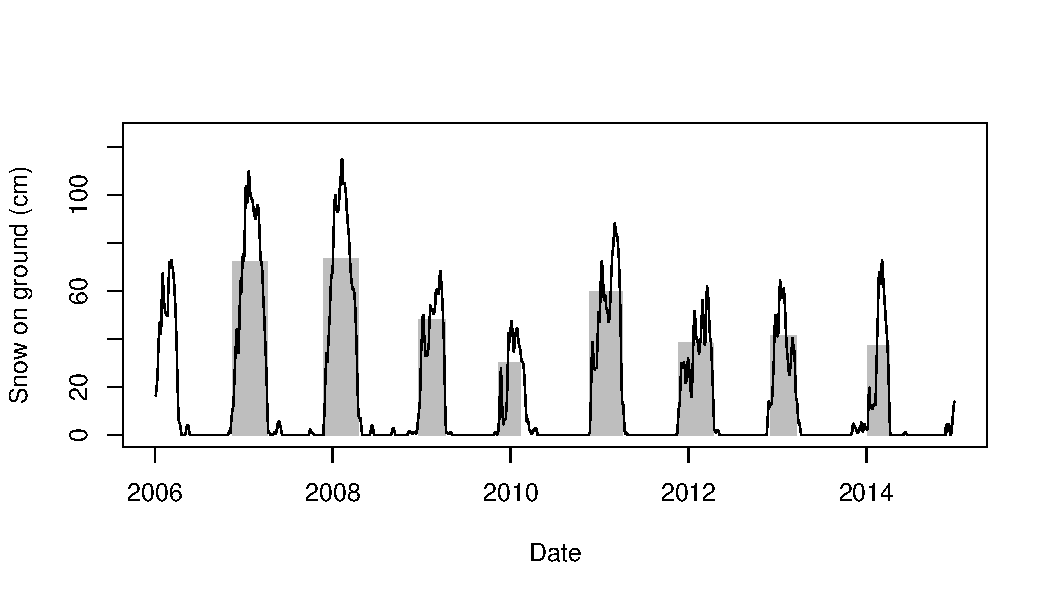
\includegraphics[width=1.0\textwidth]{report-barplots}
\end{center}
\vspace{-8mm}
\caption{Amount of snow on the ground; Lines represent the actual amount of snow at each point in the year; Bars represent the average amount of snow over the winter season.}
\label{fig:barplots}
\end{figure}


\section{Conclusion}

We used regression, time series techniques, and correlation to answer our questions. We found that the winter season starts around December 3 and ends around March 26. On average, the peak snowfall in the winter season is 86 cm and occurs around February 12. The average amount of snow present during the winter is 50 cm. We were not able to fully explain why some winters have more snow then others. Although, this can be partly explained by the temperature (which has a correlation of -0.15 with the snowfall) there are likely other factors, such as wind and precipitation that affect the amount of snowfall. Answering this kind of question would be an area for future work.

We found that the snowfall has been trending downwards at a rate of 4.42 cm per year based on our data from 2006--2014. However, there is strong uncertainty as to whether future snowfall trends can be accurately predicted. Such an analysis could possibly be done using a seasonal ARIMA model. This is also an area for future work.

In summary, we performed exploratory analysis to understand patterns in the Whistler weather data over 2006--2014. 

\nocite{*}
\bibliography{sources}

\section{Contributors}

The report was a collaborative effort. Most of the report was written with all group members present, and members edited each others work. With this in mind, the following table gives a general indication of who wrote the majority of each section.

\begin{table}[ht]
\centering
\begin{tabular}{p{9.5cm} p{6cm}}
\hline
Section & Author \\ \hline
Summary: Background, Methods, Interpretation & Nathan Esau \\
Summary: Results & Benjamin Chan \\
Introduction: Background on Whistler and data set  & Ethan Sim \\
Introduction: Imputation & Nathan Esau \\
Methods and Results: Trend & Benjamin Chan \\ 
Methods and Results: Average Smoothing & Ethan Sim \\
Methods and Results: Winter length and severity & Nathan Esau (to end of page 6), Benjamin Chan (to end of page 7) \\
Conclusion &  Ethan Sim \\ \hline
\end{tabular}
\caption{Breakdown of report by group member}
\end{table}

\medskip\noindent The code and figures, as well as the typesetting of the report were done by Nathan Esau using R and Latex.

\end{document}
